\FloatBarrier
\begin{figure}[!h]
\centering
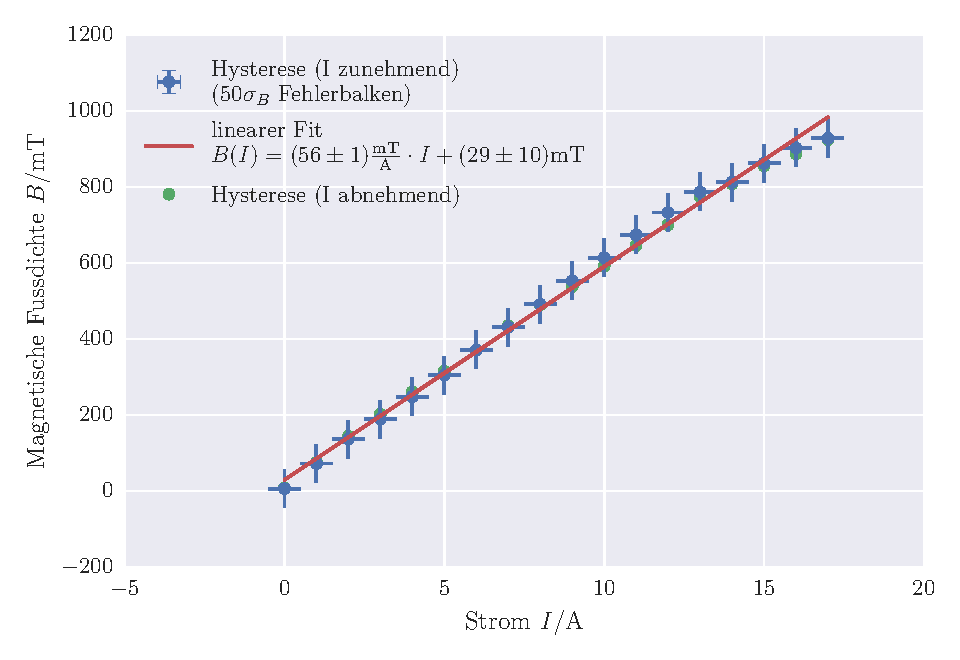
\includegraphics[scale=1]{../Grafiken/Hysterese_Messung_I_zunehmend.pdf}
\caption{Grafische Darstellung der in Abhängigkeit von der Stromstärke $I$
         aufgenommenen Messwerte der magnetischen Flussdichte $B$.
         Die zusätzlich dargestellte Regressionsgerade wurde aus den mit
         Fehlerbalken dargestellten Messwerten (für zunehmenden Strom) bestimmt.
         Die übrigen Messwerte (für abnehmenden Strom) sind für den Vergleich
         der beiden Messreihen dargestellt.
         \label{fig:hysterese_messung_i_zunehmend}}
\end{figure}
\FloatBarrier
